\documentclass{beamer}
% \documentclass[handout]{beamer}   % Für Handouts
%   \mode<handout>{%
%   \usepackage{pgfpages}
%   \pgfpagesuselayout{2 on 1}[a4paper,border shrink=5mm]
% }

\hypersetup{colorlinks=true,urlcolor=blue,linkcolor=blue}

\usepackage[T1]{fontenc}
\usepackage[utf8]{inputenc}
\usepackage[ngerman]{babel}
\usepackage{graphicx}
\usepackage{booktabs}
\usepackage{csquotes}

\setbeamertemplate{navigation symbols}{}

\AtBeginSection{
  \frame{\tableofcontents[currentsection]}
}

\begin{document}

\title{Wikischulung}
\subtitle{Gemeinsame Wissensverwaltung per Wiki}
\author{Norman Schwirz}
\institute{StuRa der HTW Dresden, Bereich Schulungen}
\titlegraphic{
\includegraphics[keepaspectratio=true, scale=1]{wikischool-logo}}
\subject{Gemeinsame Wissensverwaltung per Wiki}
\keywords{Wiki, Schulung, StuRa, Einarbeitung}
\date{\today}

\begin{frame}
  \begin{center}
    
\includegraphics[keepaspectratio=true, scale=1]{wikischool-logo}
    \begin{tabular}{|l|l|}
      \toprule
      \textbf{Thema:} & \textbf{Gemeinsame Wissensverwaltung per Wiki} \\
      \midrule
       Ort:           & KoSe 2015, Burg Hohenstein \\ 
       Datum:         & 10.01.2015 \\
       Zeit:          & 15:00 Uhr \\ 
       Referent:      &  \href{http://www.stura.htw-dresden.de/members/NormanSchwirz}{Norman Schwirz}  \\ 
      \bottomrule
    \end{tabular}
  \end{center}
\end{frame}

\begin{frame}
  \frametitle{Eure Erwartungen?}
  
  \onslide<+->
  
  \begin{center}
    
\includegraphics[width=0.7\linewidth]{500px-Notepad_icon}
  \end{center}
\end{frame}

\begin{frame}
  \frametitle{Inhalt}
  \tableofcontents
\end{frame}

\section{Was sind Wikis?}

\begin{frame}
  \frametitle{Was sind Wikis?}

  \onslide<+->
  
  % ZU VIEL TEXT!
  
  \begin{block}{}
    {\small \enquote{Ein Wiki (hawaiisch für \enquote{schnell}), seltener auch
        WikiWiki oder WikiWeb genannt, ist ein Hypertext-System für Webseiten,
        deren Inhalte von den Benutzern nicht nur gelesen, sondern auch online
        direkt im Webbrowser geändert werden können (Web-2.0-Anwendung). Diese
        Eigenschaft wird durch ein vereinfachtes Content-Management-System, die
        sogenannte Wiki-Software oder Wiki-Engine, bereitgestellt. Zum
        Bearbeiten der Inhalte wird meist eine einfach zu erlernende
        vereinfachte Auszeichnungssprache verwendet. Die bekannteste Anwendung
        ist die Online-Enzyklopädie Wikipedia, welche die Wiki-Software
        MediaWiki einsetzt.}  \\
      Quelle: \url{http://de.wikipedia.org/wiki/Wiki}, Stand 08.01.2014}
  \end{block}
  
  \begin{block}{}
    Ein Wiki bezeichnet also eine \textbf{Onlineplattform}, die mittels
    Computer \textbf{zur gemeinsamen Wissensverwaltung} genutzt werden
    kann.
  \end{block}
\end{frame}

\begin{frame}
  \frametitle{Einige Wikis im Vergleich}

  \onslide<+->
  
  \begin{columns}[t]
    
    \begin{column}{0.5\linewidth}
      \textbf{\href{http://wiki.stura.htw-dresden.de}{StuRa-Wiki}}
      \begin{itemize}
        \item Typ: MediaWiki
        \item Zweck: Das StuRa-Wiki soll KEIN Lexikon sein, sondern unserer
          Archivierung dienen
      \end{itemize}
    \end{column}

    \begin{column}{0.5\linewidth}
      \textbf{\href{http://www.wikipedia.de}{Wikipedia}}
      \begin{itemize}
        \item Typ: MediaWiki
        \item Zweck: Das Wissen der Welt sammeln und jedermann weltweit frei zur
          Verfügung stellen
      \end{itemize}
    \end{column}
  \end{columns}

  \bigskip

  \begin{columns}[t]
    \begin{column}{0.5\linewidth}
      \textbf{\href{http://www.the-empire.de}{the-empire-Wiki}}
      \begin{itemize}
        \item Typ: Semantic-MediaWiki
        \item Zweck: Organisations- und Kommunitationsplattform einer
          öffentlichen Initiative \\
      \end{itemize}
    \end{column}

    \begin{column}{0.5\linewidth}
      \textbf{\href{http://www2.htw-dresden.de/~s70341/cgi-bin/dokuwiki/doku.php}
        {Mein MitschriftenWiki}}
      \begin{itemize}
        \item Typ: DokuWiki
        \item Zweck: Gemeinsames Erstellen von Studienmitschriften als
          \emph{freies} Wissen (s.a.  Open Educational Ressources; es wird die
          gleich Lizenz wie bei der Wikipedia verwendet)
      \end{itemize}

    \end{column}
  \end{columns}
\end{frame}

% \begin{frame}
%   \frametitle{Einige Wikis im Vergleich II}

%   \onslide<+->
  
%   \begin{columns}
%     \begin{column}{0.5\linewidth}

%       \textbf{StuRa-Wiki}
%       \begin{itemize}
%       \item Typ: MediaWiki Funktionsumfang: an StuRa- Alltag angepasst, einfach
%         und ohne überflüssige Funktionen
%       \end{itemize}

%       \textbf{the-empire- Wiki}
%       \begin{itemize}
%       \item Typ: Semantic-MediaWiki Funktionsumfang: Ähnlich Mediawiki, jedoch
%         mit einigen Zusatzfunktionen (dyn. Landkarten...)
%       \end{itemize}
%     \end{column}
    
%     \begin{column}{0.5\linewidth}
    
%       \textbf{Wikipedia}
%       \begin{itemize}
%       \item Typ: MediaWiki Funktionsumfang: gemacht um das (gesamte) Wissen der
%         Welt zu speichern - von allen für alle
%       \end{itemize}

%       \textbf{MitschriftenWiki}
%       \begin{itemize}
%       \item Typ: DokuWiki Funktionsumfang: Angepasst an Studienalltag und den
%         Hochschulserver, auf dem es läuft
%       \end{itemize}
%     \end{column}
%   \end{columns}
% \end{frame}

\section{Grundsätzliche Hinweise}

\begin{frame}
  \frametitle{Grundsätzliche Hinweise}
  \framesubtitle{Haftung für Inhalte}

  \begin{center}
    
\includegraphics[scale=0.25]{Warning_256px}
  \end{center}
 
  Wikiartikel werden i.d.R offen erstellt und haben weder eine direkte
  redaktionelle Begleitung noch eine ständige Kontrolle. Auch wenn zahlreiche
  Aktive ständig an ihrer Verbesserung arbeiten, können Beiträge falsch sein und
  möglicherweise gefährdende Empfehlungen enthalten.

  \bigskip

  Daher sollte möglichst immer sorgsam, mit gesundem
  Menschenverstand und als angemeldeter Nutzer gearbeitet werden...
\end{frame}

\section{Theorie oder Praxis? (Je nach Wunsch)}

\begin{frame}
  \frametitle{Funktionsweise am Beispiel eines Mediawikis}
  \framesubtitle{Die Startseite des Wikis}

  \begin{itemize}[<+->]
    \item Die Begrüßungseite des Wikis:
    \begin{itemize}
      \item z.B.: \url{http://wiki.stura.htw-dresden.de}
    \end{itemize}
    \item wozu Anmelden?
    \begin{itemize}
      \item bessere Zuordenbarkeit von Einträgen
      \item Zugriff auf nichtöffentliche Bereiche
      \item individuelle Einstellungen
      \item Empfangen und Senden von Benachrichtigungen
    \end{itemize}
  \end{itemize}
\end{frame}

\begin{frame}
  \frametitle{Die Suchmaske}

  \begin{columns}
    \begin{column}{0.3\linewidth}
      \begin{center}
        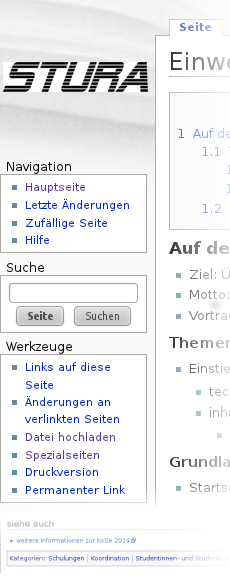
\includegraphics[width=\linewidth]{Stura-Wiki-Seitenleiste}
      \end{center}
    \end{column}

    \begin{column}{0.7\linewidth}
      \begin{itemize}[<+->]
      \item Suchen und finden
        \begin{itemize}
        \item für konkrete Suchbegriffe
        \end{itemize}
      \item Kategorien und Unterkategorien
        \begin{itemize}
        \item für thematische Suchen
        \end{itemize}
      \item Übersichtsseiten z.B.:
        \begin{itemize}
        \item \href{http://wiki.stura.htw-dresden.de/index.php/Kategorie:Abk\%C3\%BCrzung}{Abkürzungsverzeichnis}
        \item Regional-\href{http://food.the-empire.de/index.php/Hauptseite}{Übersichtsseite}
        \end{itemize}
      \item etc.
      \end{itemize}
    \end{column}
  
  \end{columns}
  
\end{frame}


\begin{frame}
  \frametitle{Die erste Bearbeitung}

  Artikel können nicht nur gelesen werden, sondern wollen auch bearbeitet
  werden - und zwar von euch!

  \begin{center}
    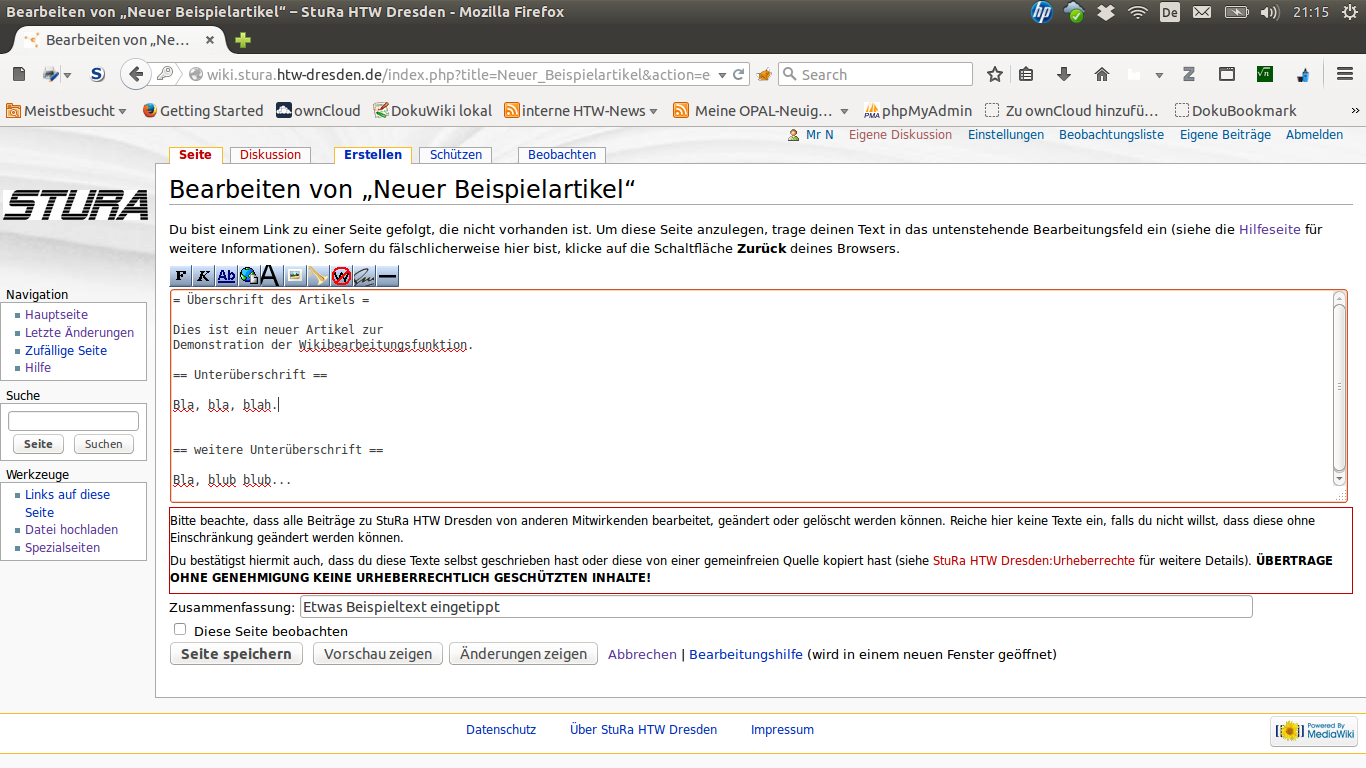
\includegraphics[width=1\linewidth]{Wikiartikel_bearbeiten}
  \end{center}
\end{frame}


\begin{frame}
  \frametitle{Die erste Bearbeitung}
  \framesubtitle{die Artikelvorschau}

  So siehts dann aus.

  \begin{center}
    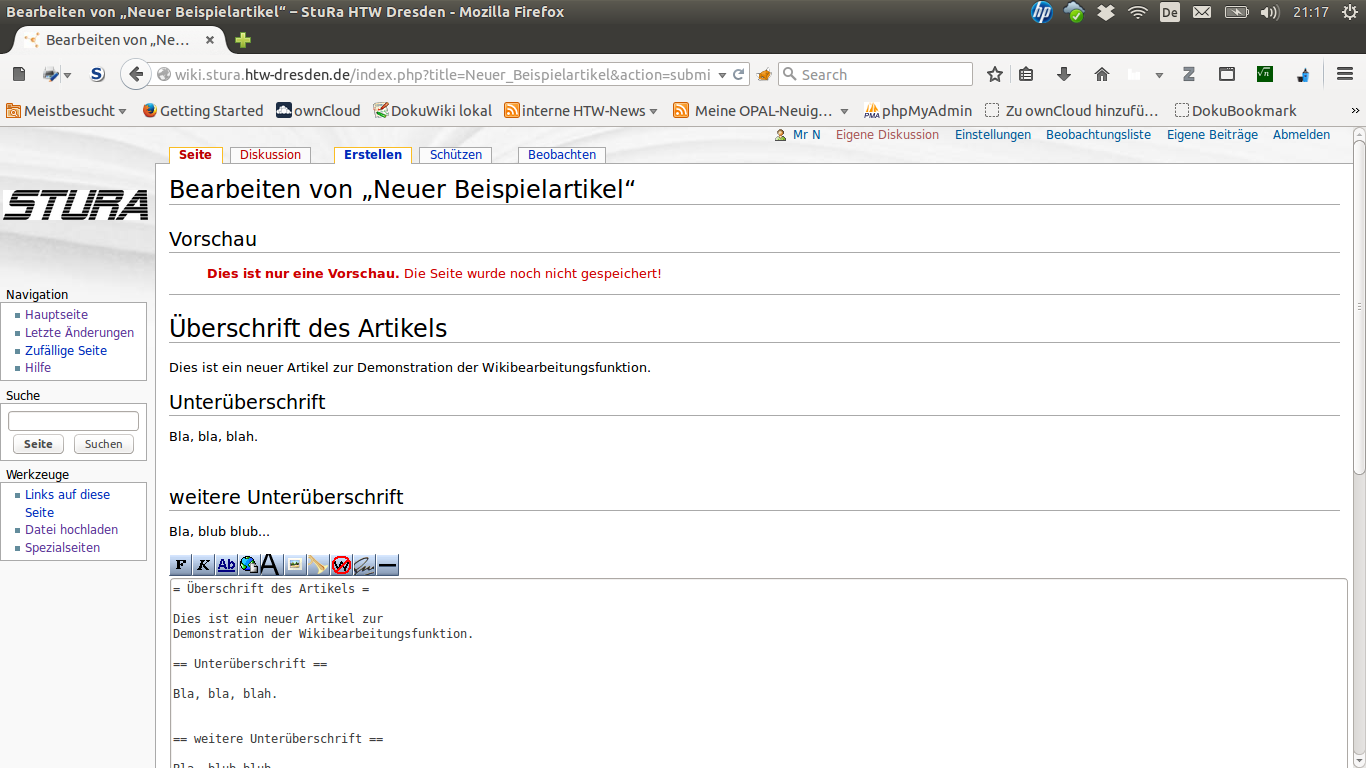
\includegraphics[width=1\linewidth]{Wikiartikel_Bearbeitungsvorschau}
  \end{center}

\end{frame}


\subsection{Wikisprache für Anfänger}

\begin{frame}
  \frametitle{Wie sag’ ich’s auf Wikiisch?}
  
  \begin{tabular}{|p{0.60\linewidth}|p{0.35\linewidth}|}
    \toprule
    \textbf{Formatierung } & \textbf{Ergebnis } \\ 
    \midrule
     
    normaler Text\newline
    (Leerzeile beginnt einen neuen Absatz) & \\ 

    \midrule
 
    \texttt{'''fettschrift'''} & \textbf{fettschrift} \\ 

    \midrule
     
    \texttt{''kursivschrift''} & \emph{kursivschrift} \\ 

    \midrule
     
    \texttt{[[Link\_auf\_eine\_Wikiseite]]}\newline
    (sog. Wikilink) & \\ 

    \midrule
    
    \texttt{[[Link\_auf\_eine\_Seite anzuzeigender\_Linktext]]}\newline
    (diesmal mit Angabe eines Textes, der anstatt des Links angezeigt wird)
                           &  anzuzeigender\_Linktext \\ 

    \midrule
     
    \texttt{[[http://www.the-empire.de Empire-Wiki]]}\newline
    (sog. externer Link) & \href{http://www.the-empire.de}{Empire-Wiki} \\ 

    \bottomrule
  \end{tabular}
  
  Zwischen den verschiedenen Wikis kann es zwar einige Unterschiede zwischen den
  Formatierungsanweisungen geben, die Art der Formatierung ist aber immer
  ähnlich.
\end{frame}


\begin{frame}
  \frametitle{Wie sag’ ich’s auf Wikiisch? II}

  \centering
  
  \begin{tabular}{|l|l|}
    \toprule
    \textbf{Formatierung } & \textbf{Ergebnis } \\ 
    \midrule
     
    Überschriften & \\ 

    \texttt{=Ebene 1=} &  Hauptüberschrift \\ 
     
    \texttt{==Ebene 2==} &  Unterüberschrift \\ 
    \midrule
     
    ungeordnete Aufzählung & \\ 

    \texttt{- Äpfel} &  *  Äpfel \\ 
    \texttt{- Birnen} &  * Birnen \\ 

    \midrule
     
    geordnete Aufzählung & \\ 
     
    \texttt{\# erstens} &  1.  erstens \\ 
    \texttt{\# zweitens} &  2.  zweitens \\ 

    \bottomrule
  \end{tabular}
\end{frame}


\begin{frame}
  \frametitle{Weitere Wiki-Formatierungen}

  \begin{center}
    \begin{tabular}{|p{0.65\linewidth}|l|}
      \toprule
      \textbf{Formatierung} & \textbf{Ergebnis} \\ 
      \midrule
      \texttt{[[Datei:Bild.jpg|Text]]} oder\newline \texttt{[[Bilddatei|miniatur|Größe|Position|Bilduntertitel]]}  &   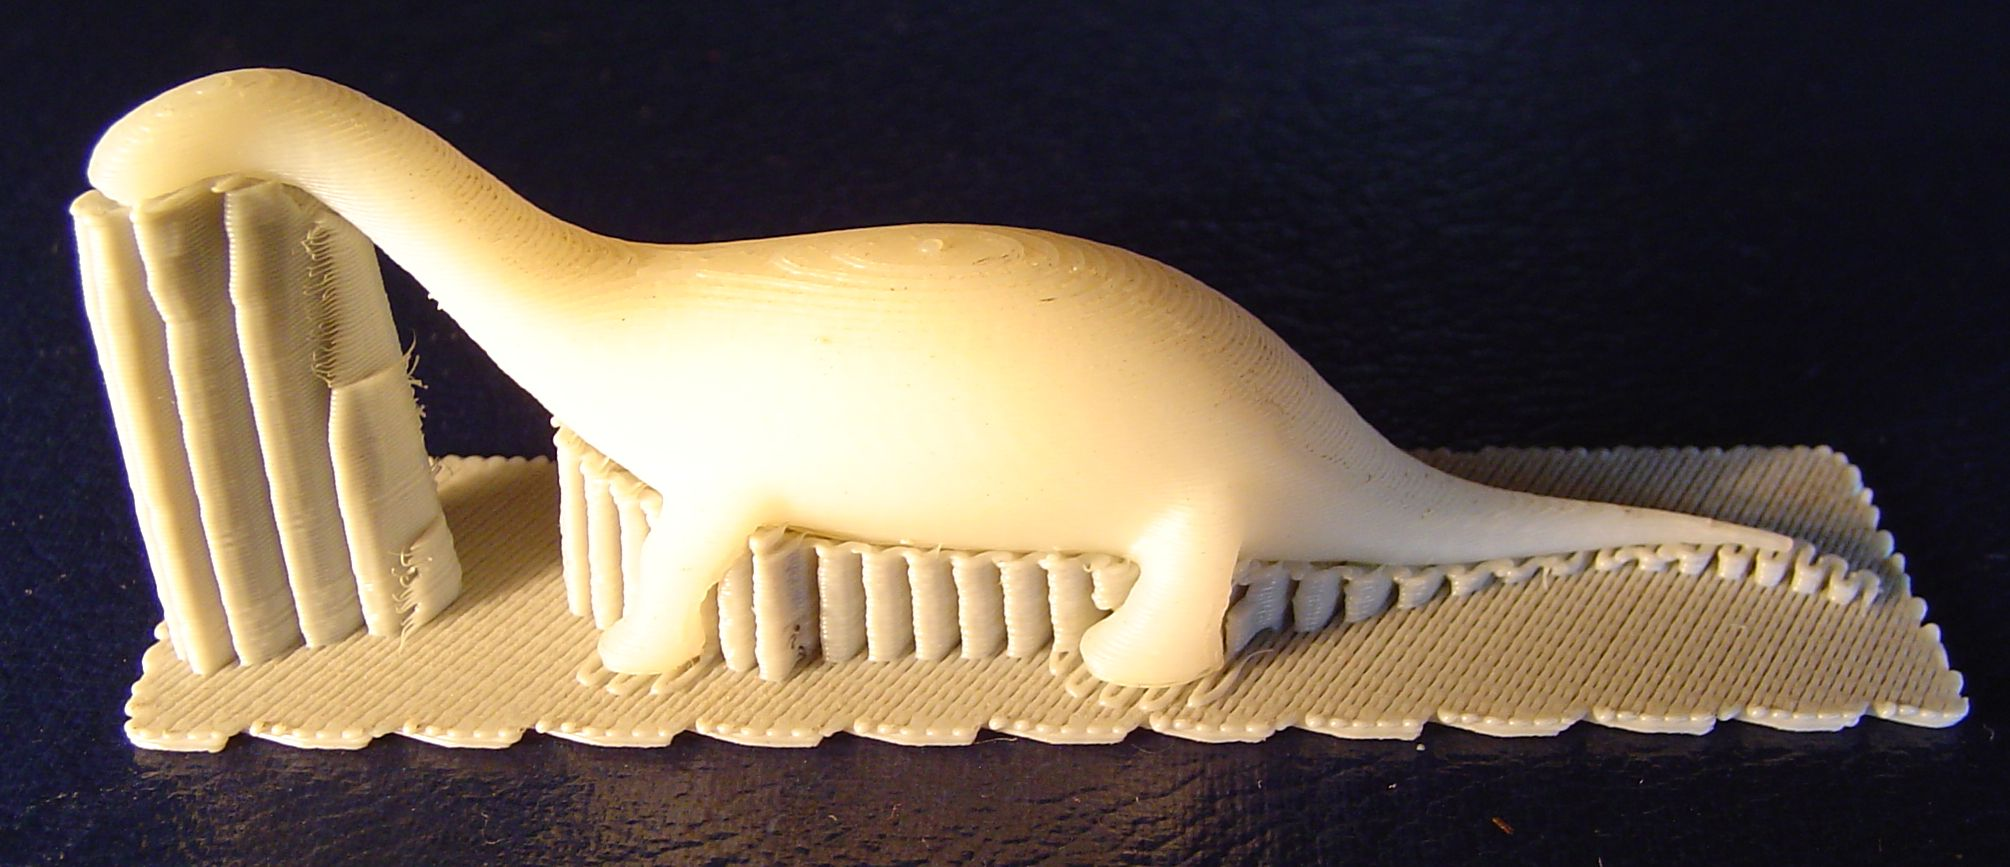
\includegraphics[keepaspectratio=true, width=0.2\textwidth]{rapid-dino.jpg} \\
      \midrule
      Tabellen & \href{https://de.wikipedia.org/wiki/Hilfe:Tabellen}{Beispiel siehe hier} \\ 
      \midrule
      % \texttt{<math> a^2 + b^2 = c^2 </math> } & Beispiel für die Matheformel $ a^2 + b^2 = c^2 $ \\
      \dots & \dots \\     
      \hline
    \end{tabular}
  \end{center}

  \bigskip
  
  Keine Sorge beim Ausprobieren! Sämtliche Änderungen sind nachvollziehbar und
  können in der Regel rückgängig gemacht werden.
\end{frame}


\begin{frame}
  \frametitle{Was sind Diskussionsseiten?}

  \begin{itemize}[<+->]
    \item sie dienen der Diskussion über den zugehörigen Artikel
    \item auf ihnen können Fragen und Ideen zur Diskussion gestellt werden,
      die im eigentlichen Artikel fehl am Platz wären
  \end{itemize}

  \begin{center}
    
\includegraphics[width=\linewidth]{Wiki-Kopfzeile_Diskussionslink_markiert}
  \end{center}

\end{frame}


\begin{frame}
  \frametitle{Wer hat was wann wie geändert?}

  Antwort auf diese Frage geben die:
  \begin{itemize}[<+->]
    \item Versionshistorie % Versionsgeschichte?
    \begin{itemize}
      \item Wann, warum und von wem wurde der aktuelle Artikel bisher bearbeitet?
    \end{itemize}
    \item Differenzenansicht
    \begin{itemize}
      \item Wie sah der Artikel früher einmal aus?
    \end{itemize}
  \end{itemize}
\end{frame}


\begin{frame}
  \frametitle{Änderungsbenachrichtigungen}

  \onslide<+->
  
  \begin{itemize}[<+->]
  \item Um sofort zu erfahren, wenn Artikel bearbeitet wurden
  \item bequem per
    \begin{itemize}
    \item Email
    \item Newsfeed
    \end{itemize}
  \item individuell abonnierbar
    \begin{itemize}
    \item z.B. per Beobachtungsliste
    \end{itemize}
  \end{itemize}

  \onslide<+->
  
  Eingeloggtes Arbeiten bringt Vorteile mit sich \dots
\end{frame}

\begin{frame}
  \frametitle{Wikilinks, Permalinks und “Links auf diese Seite”}
  
  \begin{itemize}[<+->]
  \item Wikiartikel können besonders einfach miteinander verknüpft werden
  \item nicht existierende Zielartikel werden beim 1. Besuch automatisch
    erstellt
  \item sog. Perma(nent)links verweisen hierbei nicht auf die aktuelle
    Artikelfassung sondern auf \textbf{eine bestimmte} frühere
  \item Doch von wo alles wird hierher verlinkt?
  \end{itemize}
  
\end{frame}


\begin{frame}
  \frametitle{Einen neuen Wikiartikel erstellen}
  
  \begin{itemize}[<+->]
    \item Vorab-Fragen
    \begin{itemize}
      \item Zweck (z.B.: Ideenfindung, Dokumentation)
      \item Sinn, gibt es bereits ähnliche Artikel
      \item Name des neuen Artikels (Singular verwenden)
    \end{itemize}
    \item Artikelerstellung
    \begin{itemize}
      \item Artikelgestaltung (Schreibstil \& Co.)
      \item ggf. Quellenangaben/ Belege anfügen
    \end{itemize}
    \item Übersichtsseite neu angelegter Artikel
  \end{itemize}

  \onslide<+->
  
  Artikel, Namespaces, Kategorien bitte in Singularform!
\end{frame}

\subsection{ein wenig zu Wiki-Aufbau und Struktur}

\begin{frame}
  \frametitle{Aufbau/Struktur des StuRa-Wikis}
  
  \begin{itemize}[<+->]
  \item
    \href{http://wiki.stura.htw-dresden.de/index.php/Spezial:Kategorien}{Kategorien}
    und
    [\url{http://wiki.stura.htw-dresden.de/index.php/Kategorie}:!Hauptkategorie/Unterkategorien]
  \item \href{http://wiki.stura.htw-dresden.de/index.php/Admin:Namensr\%C3\%A4ume}{Namensräume}
  \item Einstiegs-/ Übersichtsseiten
    \begin{itemize}
    \item \href{http://wiki.stura.htw-dresden.de/index.php/Hauptseite}{Startseite} des Wikis
    \item \href{http://wiki.stura.htw-dresden.de/index.php/StuRa_HTW_Dresden:Erste_Schritte}{Erste Schritte} (!)
    \item Einarbeitungsseiten
      (\href{http://wiki.stura.htw-dresden.de/index.php/Wiki/Einarbeitung}{Wiki},
      \href{http://wiki.stura.htw-dresden.de/index.php/Einarbeitung}{Allgemein})
    \item Infos zur
      \href{http://wiki.stura.htw-dresden.de/index.php/Artikelerstellung}{Artikelerstellung}
      und
      \href{http://wiki.stura.htw-dresden.de/index.php/Admin:Artikelgestaltung}{-gestaltung}
      sowie
      \href{https://de.wikipedia.org/wiki/Wikipedia:Wie_schreibe_ich_gute_Artikel}{weitereTipps}
    \end{itemize}
  \item Spezialseiten
  \end{itemize}
\end{frame}

\subsection{der erste selbst erstellte Wikiartikel}

\begin{frame}
  \frametitle{Zeit für die Praxis...}
  \framesubtitle{der erste eigene Wikiartikel}

  Bestimmt hast du dir schon einen Wikiartikel ausgesucht, den du erweitern oder
  aktualisieren möchtest. Natürlich kannst du auch einen neuen Wikiartikel
  Erstellen.
  
  \begin{itemize}
  \item Wikiartikel bearbeiten- Link
  \item neuen Wikiartikel anlegen
    \begin{itemize}
    \item \emph{Artikel-Wunschliste}: Einen Artikel aus der Liste "gewünschter"
      Wikiartikel anlegen
    \item \emph{Wikilink verwenden}: Einfach in einem bestehenden Wikiartikel
      auf einen \texttt{[[neuen Wikiartikel]]} verlinken (er wird dann beim
      1. draufklicken automatisch erstellt)
    \end{itemize}
  \end{itemize}

\end{frame}

\begin{frame}
  \frametitle{Bilder und andere Medien}
  \framesubtitle{ins Wiki hochladen und verwenden}

\end{frame}


\begin{frame}
  \frametitle{Bilder und andere Medien}
  \framesubtitle{aktualisieren und kommentieren}

\end{frame}


\begin{frame}
  \frametitle{Spezialseiten}
%%  \framesubtitle{}

\end{frame}

\section{Was gehört ins Wiki und was nicht?}

\begin{frame}
  \frametitle{Was gehört (nicht) ins Wiki?}

\end{frame}

  
\begin{frame}
  \frametitle{Was sollte nun klar sein?}
  \begin{itemize}[<+->]
    \item Was Wikis sind und wie man sie benutzt
    \item Wie aus einer Idee ein Wikiartikel werden kann, der uns allen nützt
    \item Wieso man auf seinen gesunden Menschenverstand hören sollte
    \item wie Wikis meist aufgebaut sind
    \item Wo bzw. wie ich Hilfe finden kann
  \end{itemize}
\end{frame}

\section{(Semantic) Mediawiki und Addons (ja nach Interesse)}

\begin{frame}
  \frametitle{Semantik MediaWiki}

  \begin{center}
    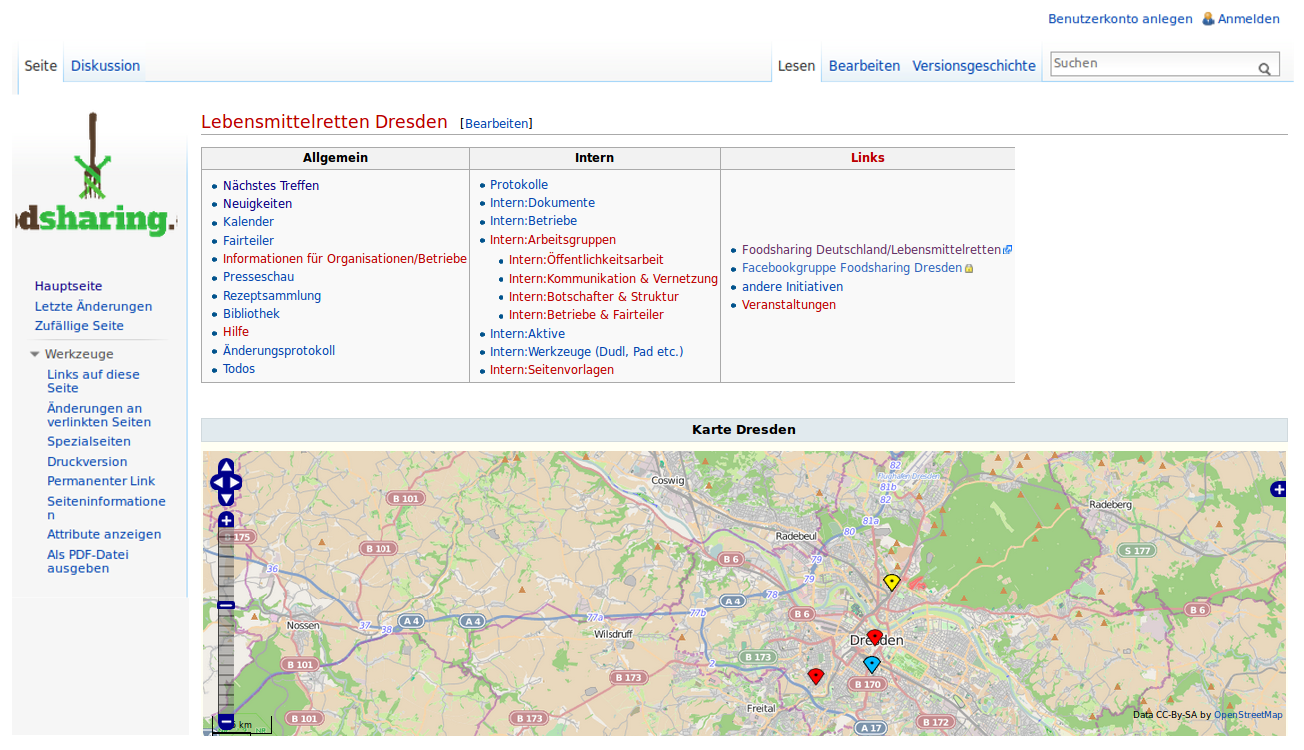
\includegraphics[width=\linewidth]
    {Lebensmittelretten-Dresden_Landkarte_mit_Seitenleisten}
  \end{center}

  \dots\ Am Beispiel von Lebensmittelretten Dresden
  (\url{http://food.the-empire.de})
\end{frame}
  
%\begin{frame}
%  \frametitle{Semantik-MediaWiki II (Semantik)}
%
%  800px|gerahmt|zentriert|...und hier noch ein [Bsp. aus dem The Empire-Wiki](http://www.the-empire.de/index.php/Spezial:Durchsuchen/Einrichtung:Aprikosengarten)
%
%\end{frame}


\begin{frame}
  \frametitle{MediaWiki-Erweiterungen (sog. Addons)}

  \begin{center}
    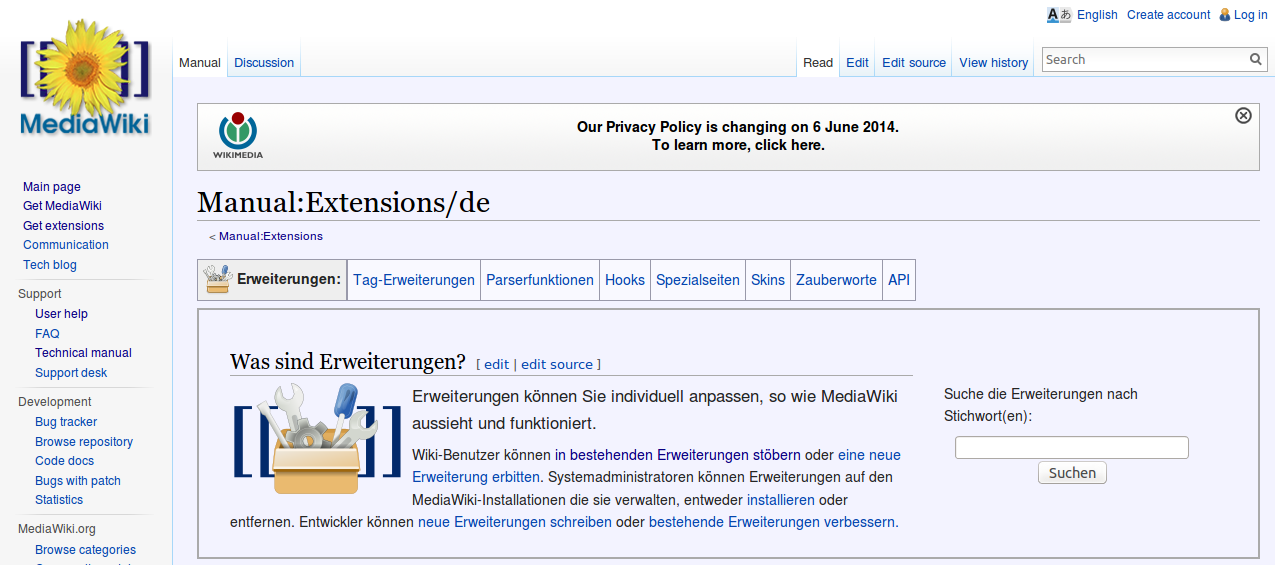
\includegraphics[width=\linewidth]{Mediawiki-Extensions}

    \medskip
    
    (\url{https://www.mediawiki.org/wiki/Manual:Extensions/de})
  \end{center}
  
\end{frame}

\section{Fragerunde}

\begin{frame}
  \frametitle{Danke für eure Aufmerksamkeit!}
  \framesubtitle{Gibts Fragen?}

  \begin{center}
    
\includegraphics[scale=0.5]{Circle-question_400x400.png}
  \end{center}

\end{frame}


\begin{frame}
  \frametitle{Quellen}

  \begin{itemize}
  \item \url{http://wiki.stura.htw-dresden.de}
  \item \url{http://www.the-empire.de}
  \item \url{http://food.the-empire.de}
  \item \url{http://www2.htw-dresden.de/~s70341/cgi-bin/dokuwiki}
  \item \url{http://www.wikipedia.org}
  \item \url{https://commons.wikimedia.org}
  \item \url{https://www.mediawiki.org/wiki/Manual:Extensions/de}
  \end{itemize}
  
\end{frame}

\begin{frame}
  \frametitle{Das Wiki ist, was ihr draus macht!}
  \framesubtitle{Link zur Präsentation}

  \begin{itemize}
  \item Wikiartikel der Schulung incl. Präsentationsfolien:\\
   \url{http://wiki.stura.htw-dresden.de/index.php/Konstituierungsseminar/2015/Wikischulung}
  \item \emph{Präsentationsfolien im Plone}:\\
    \url{http://www.stura.htw-dresden.de/stura/ref/verwaltung/schulungen/kose/kose-2015/praesentationen/wiki-schulung-kose-2015}
  \item \emph{LaTeX-Quelldateien zum Überarbeiten}:\\
    \url{https://github.com/Nos-/Studium/tree/master/Wikivortrag}
  \end{itemize}
  
\end{frame}

\end{document}

%%% Local Variables:
%%% mode: latex
%%% TeX-master: t
%%% End:
